\mainmatter%
\setcounter{page}{1}

\lectureseries[\course]{\course}

\auth[\lecAuth]{Lecturer: \lecAuth\\ Scribe: \scribe}
\date{November 12, 2009}

\setaddress%

% the following hack starts the lecture numbering at 13
\setcounter{lecture}{12}
\setcounter{chapter}{12}

\lecture{Open Loop Control}

\section{Open Loop is Feedback}
The dynamics and initial conditions are given by
\begin{align}
\label{eq:13d}
\dot{\xi} &= f(\xi,u) \\
\label{eq:13ic}
\xi_s &= x
\end{align}
The open loop control space is

\begin{equation*}
\mathcal{U}_{s,t} = \left\lbrace u:[s,t)\to\mathcal{U}\subseteq \mathbb{R}^k~|~\int_s^t |u_t|^2dt < \infty \right\rbrace% chktex 9
\end{equation*}

and the closed loop, or feedback, control space is

\begin{equation*}
\mathcal{M}_{s,t} = \left\lbrace \mu:[s,t)\times\mathbb{R}^n\to\mathcal{U}\subseteq\mathbb{R}^k~|~\int_s^t |\mu_t(\xi_t)|^2dt < \infty~\forall x \in \mathbb{R}^n \right\rbrace% chktex 9
\end{equation*}

given that there exists a unique solution to (\ref{eq:13d}) and (\ref{eq:13ic}).
The cost function mapping is $J:[0,T]\times\mathbb{R}^n\times\mathcal{U}_{s,t}\to\mathbb{R}$ and the cost function is
\begin{align}
\label{eq:13cost}
J(s,x,u) = \int_s^T l(\xi_t,u_t)dt + \vp(xi_t)
\end{align}
The value function is

\begin{equation*}
V(s,x) = \inf_{\uinu}J(s,x,u)
\end{equation*}

and the feedback versions are
\begin{align*}
&J^F: [0,T)\times\mathbb{R}^n\times\mathcal{M}_{s,t}\to\mathbb{R} \\% chktex 9
&J^F(s,x,\mu) = \int_s^T l(\xi_t,\mu_t(\xi_t))dt + \psi(\xi_t) \\
&V^F(s,x) = \inf_{\mu\in\mathcal{M}_{s,T}}J^F(s,x,\mu)
\end{align*}

\begin{proposition}%
\label{prop:13value}

\begin{equation*}
V(s,x) = V^F(s,x)~\forall s\in[0,T),~\forall x\in\mathbb{R}^n% chktex 9
\end{equation*}

\end{proposition}

\begin{proof}
We need to show that $V(s,x)\leq V^F(s,x)$ and $V(s,x)\geq V^F(s,x)$ which would make them equal.
  To show $V(s,x)\leq V^F(s,x)$ let $u^\epsilon$  be $\epsilon$-optimal for $V$, i.e.,
\begin{align}
\label{eq:13optimal}
J(s,x,u^\epsilon) \leq V(s,x) + \epsilon
\end{align}
Note that open loop is feedback control that does not pay attention to the state.
Then, let $\tilde{\mu}_t(x) \doteq u_t^\epsilon~\forall x,~\forall t$.
This gives
\begin{align}
\label{eq:13feedback}
V^F(s,x) \leq J^F(s,x,\tilde{\mu}) = F(s,x,u^\epsilon)
\end{align}
By (\ref{eq:13optimal}) and (\ref{eq:13feedback}) we see that $V^F(s,x)\leq V(s,x)+\epsilon$ is true for all $\epsilon$, therefore $V^F\leq V$.

To show $V(s,x)\geq V^F(s,x)$ let $\mu^\epsilon$ be $\epsilon$-optimal for $V^F$, i.e.,
\begin{align}
\label{eq:13costeps}
J^F(s,x,\mu^\epsilon)\leq V^F(s,x) + \epsilon
\end{align}
Let $\xi^\epsilon$ be the unique solution of
\begin{align}
\label{eq:13state}
\dot{\xi}=f(\xi_t,\mu_t^\epsilon(\xi_t))
\end{align}
with $\xi_s=x$.
Let $\hat{u}_t=\mu_t^\epsilon(\xi_t^\epsilon)~\forall t$.
Then let $\xi^\epsilon$ be the solution of
\begin{align}
\label{eq:13stateeps}
\dot{\xi}^\epsilon = f(\xi_t^\epsilon,\hat{u}_t)
\end{align}
where again $\xi_s=x$.
Now we let $\bar{\xi}$ be the unique solution of $\dot{\xi}_t=f(\xi_t,\hat{u}_t)$.
Then, by (\ref{eq:13state}) and (\ref{eq:13stateeps}) $\bar{\xi}=\xi^\epsilon$.
Therefore
\begin{align}
\label{eq:13valueeps}
V(s,x) \leq J(s,x,\hat{u}) = J^F(s,x,\mu^\epsilon)
\end{align}
Finally, by (\ref{eq:13costeps}) and (\ref{eq:13valueeps}) we find that

\begin{equation*}
V(s,x) \leq V^\epsilon(s,x)
\end{equation*}

\end{proof}

This shows that if the system is deterministic then we can predict the trajectory using open loop control, so feedback is open loop control.
However, we know that real systems have noise in them.
The open loop controller is still useful because it is easier to solve than the feedback controller and the open loop controller can be used iteratively such that when the system gets to a state we know is wrong the open loop controller can be reset.

How do we know $\mu^\epsilon\in\mathcal{M}_{s,t}$? This goes back to $|f(x,u)-f(y,u)|\leq K|x-y|$ and knowing that we get a unique solution.

\section{Open Loop Control}
Let $u\in\mathcal{U}_{s,T}$, $\tau\in(s,T)$ and $u^0:[s,\tau)\to\mathcal{U}$.% chktex 9
This is given by $u^0=u_t~\forall t\in[s,\tau)$.% chktex 9
Then we have the mapping $u^1: [\tau,T)\to\mathcal{U}$ and get that $u^1_t=u_t~\forall t\in[\tau,T)$.% chktex 9
This leads to $u^0\in\mathcal{U}_{s,\tau}$ and $u^1\in\mathcal{U}_{\tau,T}$.
Letting

\begin{equation*}
u_t=\begin{cases} u_t^0, & t\in[s,\tau) \\ u_t^1, & t\in[\tau,T) \end{cases}% chktex 9
\end{equation*}

we get $u\in\mathcal{U}_{s,T}$.
See Figure~\ref{fig:13controlspace}.

\begin{figure}[ht!]
\centering
\includegraphics[width=.5\textwidth]{images/13controlspace}
\caption{Multiple control spaces.}%
\label{fig:13controlspace}
\end{figure}

\section{Dynamic Programming Principle}
Now we want to find the DPP using the value function.
We get that
\begin{align*}
V(s,x) &= \inf_{u\in\mathcal{U}_{s,T}} \left\lbrace \int_s^T l(\xi_t,u_t)dt + \vp(\xi_t) \right\rbrace \\
&= \inf_{u^0\in\mathcal{U}_{s,\tau}} \inf_{u^1\in\mathcal{U}_{\tau,T}} \left\lbrace \int_s^\tau l(\xi_t,u_t^0)dt + \int_\tau^T l(\xi_t,u_t^1)dt + \vp(\xi_t) \right\rbrace
\end{align*}
where $\xi$ satisfies (\ref{eq:13d}) and (\ref{eq:13ic}) with control $u$.
This gives
\begin{align*}
V(s,x) = \inf_{u^0\in\mathcal{U}_{s,\tau}} \left\lbrace \int_s^\tau l(\xi^0,u_t^0)dt + \inf_{u^1\in\mathcal{U}_{\tau,T}} \left[\int_\tau^T l(\xi^1,u_t^1)dt + \vp(\xi_t^1)\right]\right\rbrace
\end{align*}
where $\xi^0$ satisfies (\ref{eq:13d}) and (\ref{eq:13ic}) for control $u^0$ and $\xi^1$ satisfies (\ref{eq:13d}) and (\ref{eq:13ic}) for control $u^1$ as seen in Figure~\ref{fig:13controlspace}.

\begin{theorem}{Dynamic Programming Principle}

$\forall \tau\in[s,T),~\forall x\in\mathbb{R}^n$ we have that% chktex 9
\begin{align}
\label{eq:13dpp}
V(s,x) = \inf_{u^0\in\mathcal{U}_{s,\tau}} \left\lbrace \int_s^\tau l(\xi^0,u^0)dt + V(\tau,\xi_\tau^0) \right\rbrace
\end{align}
where $\xi^0$ satisfies (\ref{eq:13d}) and (\ref{eq:13ic}) for control $u^0$.
\end{theorem}

\section{Dynamic Programming Equation}
The DPE will be the Hamilton, Jacobi, Bellman (HJB) partial differential equation (PDE).
To go from the DPP to the DPE there are two methods available.
\begin{itemize}
\item Use DPP, let $\tau\downarrow s$, then show that $V$ is the solution of the HJB PDE\@.
      We would still need uniqueness for HJB PDE\@.
\item It can be found in the literature that there exists a unique solution to the HJB PDE\@.
      The next step would be to show that it must be $V$.
\end{itemize}

\subsection{Method 1}
From (\ref{eq:13dpp}) we have
\begin{align}
\label{eq:13method1}
\begin{split}
0 &= \inf_{u^0\in\mathcal{U}_{s,\tau}} \left\lbrace \frac{\int_s^\tau l(\xi_t,u_t^0)dt}{\tau-s} + \frac{V(\tau,\xi_t)-V(s,x)}{\tau-s} \right\rbrace \\
&\approx\inf_{v\in\mathcal{U}} \left\lbrace \frac{\int_s^\tau l(\xi_t,v)dt}{\tau-s} + \frac{V(\tau,\xi_t)-V(s,x)}{\tau-s} \right\rbrace
\end{split}
\end{align}
As $\tau\downarrow s$
\begin{align}
\label{eq:13limit}
\frac{\int_s^\tau l(\xi_t,v)}{\tau-s} \to l(x,u)
\end{align}
Also, using Taylor series expansion
\begin{align*}
V(\tau,\xi_t) &= V(s,x) + \left.\frac{d}{dt}V(t,\xi_t)\right|_{t=s}(\tau-s) + \mathcal{O}(|\tau-s|^2) \\
&= V(s,x) + V_s(s,x) + \nabla_x V(s,x) \left.\frac{d\xi_t}{dt}\right|_{t=s}(\tau-s) + \mathcal{O}(|\tau-s|^2)
\end{align*}
\begin{align}
\label{eq:13valtaylor}
\Rightarrow \frac{V(\tau,\xi_\tau)-V(s,x)}{\tau-s} &= \left[V_s(s,x) + \nabla_x V(s,x)F(x,u)\right] + \mathcal{O}(|\tau-s|)
\end{align}
By (\ref{eq:13method1}), (\ref{eq:13limit}) and (\ref{eq:13valtaylor}) and letting $\tau\downarrow s$
\begin{align*}
0 &= \inf_{\uinu} \left\lbrace l(x,u) + V_s(s,x) + \nabla_x V(s,x)f(x,u) \right\rbrace \\
0 &= V_s(s,x) + \underbrace{\inf_{\uinu} \left\lbrace l(x,u) + \nabla_x V(s,x)f(x,u) \right\rbrace}_{\text{Hamiltonian}}
\end{align*}
This is the DPE for the HJB PDE\@.

Recall the definition of the value function

\begin{equation*}
V(s,x) = \inf_{u\in\mathcal{U}_{s,T}} J(s,x,u)
\end{equation*}

This shows that $V(T,x) = \vp(x)$ is the terminal cost.
Then

\begin{equation*}
\mu^\ast \in \arg\min_{\uinu} \left\lbrace l(x,u) + \nabla_x V(s,x) f(x,u) \right\rbrace
\end{equation*}

Notice that this is feedback control even though we started looking at open loop control, which makes sense because of Proposition~\ref{prop:13value}.

\begin{example}%
\label{ex:13hjb}
Let the dynamics and initial conditions be
\begin{align*}
\dot{\xi} &= \sqrt{|\xi_t|}\cdot \text{sign}(\xi_t)u_t \\
\xi_s &= x
\end{align*}
The cost is

\begin{equation*}
J(s,x,u) = \int_s^T |\xi_t|+u_t^2dt
\end{equation*}

where $\psi=0$ means there is no terminal payoff.
The HJB PDE is found as

\begin{equation*}
0 = V_s(s,x) + \inf_{v\in\mathbb{R}} \underbrace{\left[|x|+v^2+\sqrt{|x|}\cdot\text{sign}(x)\cdot v\right]}_{g(v)}
\end{equation*}

Notice that $g(v)$ is quadratic and is a typical way of setting up these types of problems.
From this we get
\begin{align*}
g^1(v) &= \partial v + V_x\sqrt{|x|}\cdot \text{sign}(x) = 0 \\
v^0 &= -\frac{V_x\sqrt{|x|}\cdot\text{sign}(x)}{2} \\
g(v^0) &= |x| + \frac{1}{4}V_x^2|x| + V_x\sqrt{|x|}\cdot\text{sign}(x) \\
&= |x| + \frac{1}{4}V_x^2|x| - \frac{V_x^2|x|}{2} \\
&= |x| - \frac{1}{4}V_x^2|x| \qquad [\text{this is the Hamiltonian}] \\
\Rightarrow 0 &= V_s + |x| - \frac{1}{4}|x|V_x^2 \\
V(T,x) &= 0
\end{align*}
Now we can guess that $V(s,x) = h(s)|x|$.
Keep in mind that the running cost, $l$, can be set by the engineer to help make these problems realistic but solvable.
So we use
\begin{align*}
V_s &= h^1(s)|x| \\
V_x &= h(s)\cdot\text{sign}(x), \qquad [x\neq0] \\
V_x^2 &= h^2(s) \\
\Rightarrow 0 &= h(s)|x| + |x| + \frac{1}{4}|x|h^2(s) \\
\frac{dh}{ds} &= -1 + \frac{1}{4}h^2(s) = \frac{h^2(s)-4}{4} \\
\frac{dh}{h^2(s)-4} &= \frac{ds}{4}
\end{align*}
For the last expression we probably need to look up the solution in integral tables.
Those yield a solution of
\begin{align*}
\frac{1}{4}\ln\left(\frac{2-h}{2+h}\right) &= \frac{s}{4} + c \\
\frac{2-h}{2+h} &= \tilde{c}e^s \\
2-h &= 2\tilde{c}e^s + h\tilde{c}e^s \\
2-2\tilde{c}e^s &= h(\tilde{c}e^s+1) \\
\Rightarrow h &= \frac{1-\tilde{c}e^s}{1+\tilde{c}e^s}
\end{align*}
By the terminal condition we get

\begin{equation*}
0 = 2(1-\tilde{c}e^T) \Rightarrow \tilde{c} = e^{-T}
\end{equation*}

Now the value function is

\begin{equation*}
V(s,x) = 2\left(\frac{1-e^{s-T}}{1+e^{s-T}}\right)|x|
\end{equation*}

Using the value function we can find the optimal control as
\begin{align*}
\mu^\ast(s,x) &= \underbrace{-2\left(\frac{1-e^{s-T}}{1+e^{s-T}}\right)\cdot\text{sign}(x)}_{V_x}\cdot\frac{\text{sign}(x)\sqrt{|x|}}{2} \\
&= \left(\frac{1-e^{s-T}}{1+e^{s-T}}\right)\sqrt{|x|}
\end{align*}
We can look at the trajectory, $\dot{\xi}^\ast$, to see if it makes sense.
\begin{align*}
\dot{\xi}^\ast &= -\left(\frac{1-e^{s-T}}{1+e^{s-T}}\right)|\xi_t^\ast|\cdot\text{sign}(\xi_t^\ast) \\
&= -\left(\frac{1-e^{s-T}}{1+e^{s-T}}\right)\xi_t^\ast
\end{align*}
Figure~\ref{fig:13trajectory} shows the trajectory which looks correct.
$\lozenge$
\end{example}

\begin{figure}[ht!]
\centering
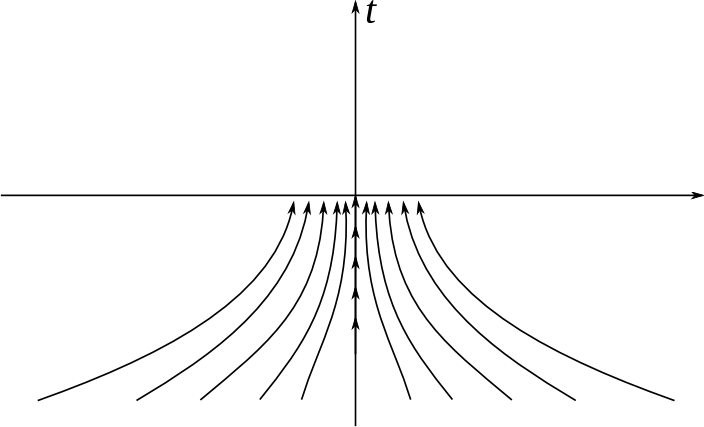
\includegraphics[width=.6\textwidth]{images/13trajectory}
\caption{State dynamics trajectory.}%
\label{fig:13trajectory}
\end{figure}% chktex 17
